%!TEX root = ../../msc17-game-book.tex


\phChapterWorksheet{Fear the Hungry Dead}{Main Puzzle 2}

The insatiable Zom Bea eats anything in her path. Last year at Count Calcula's party she ate ALL of the Count's famous meat pie! She started by eating half of the pie... then she ate half of the remaining pie! Actually, she
continued to have more and more servings, each time eating half of the
remaining pie.

Here's a picture to give you the idea. (Hey, what kind of monster bakes
a square pie, though?)

\begin{center}
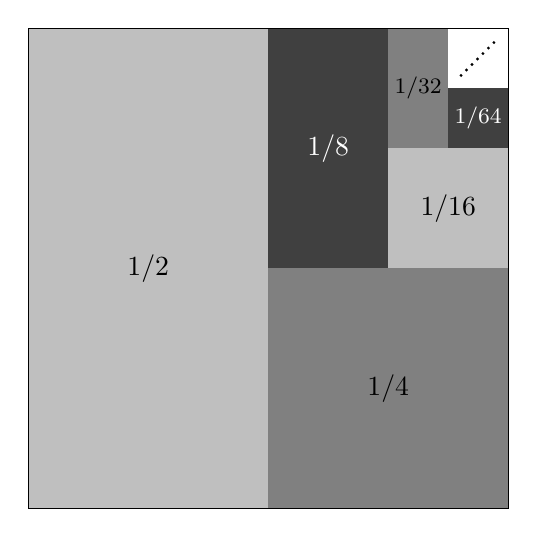
\begin{tikzpicture}[x=0.3in,y=0.3in]
  \fill[color=lightgray] (0,0) rectangle (4,8) node[pos=.5,color=black] {1/2};
  \fill[color=gray] (4,0) rectangle (8,4) node[pos=.5,color=black] {1/4};
  \fill[color=darkgray] (4,4) rectangle (6,8) node[pos=.5,color=white] {1/8};
  \fill[color=lightgray] (6,4) rectangle (8,6) node[pos=.5,color=black] {1/16};
  \fill[color=gray] (6,6) rectangle (7,8)  node[pos=.5,color=black] {\footnotesize 1/32};
  \fill[color=darkgray] (7,6) rectangle (8,7) node[pos=.5,color=white] {\footnotesize 1/64};
  \draw[thick,dotted] (7.2,7.2) -- (7.8,7.8);
  \draw (0,0) rectangle (8,8);
\end{tikzpicture}
\end{center}

Since there was no pie left for anyone else, the Count has given Zom some
stipulations for the amount she is allowed to eat this year.
(Otherwise, guess who isn't getting invited to any future parites!) The Count
has made it clear: ``Zom's first serving must be
no larger than \(\frac{1}{4}\) the entire pie, and any future serving cannot
be larger than \(\frac{1}{4}\) the most recent serving!''

Zom is terrified that this delicious meat pie will be her last, so maybe you can
help her out. \textbf{What fraction of the pie is she allowed to eat?}
\textbf{Make sure you draw a picture which explains why.}
Bear in mind, she feels like she could eat servings of the delectible
pie \textit{forever}.

Oh, and Zom doesn't know what shape the pie will be this year, but does
it matter?
